\documentclass[10pt,conference,onecolumn,compsoc]{IEEEtran}
\usepackage{float}

\usepackage{blindtext}
\usepackage{subcaption}

\usepackage{hyperref}
\usepackage{enumitem}
\setlist[itemize]{leftmargin=3 cm}
\setlist[enumerate]{leftmargin=3cm}



% *** CITATION PACKAGES ***
%
\ifCLASSOPTIONcompsoc
  % IEEE Computer Society needs nocompress option
  % requires cite.sty v4.0 or later (November 2003)
  \usepackage[nocompress]{cite}
\else
  % normal IEEE
  \usepackage{cite}
\fi
% cite.sty was written by Donald Arseneau
% V1.6 and later of IEEEtran pre-defines the format of the cite.sty package
% \cite{} output to follow that of IEEE. Loading the cite package will
% result in citation numbers being automatically sorted and properly
% "compressed/ranged". e.g., [1], [9], [2], [7], [5], [6] without using
% cite.sty will become [1], [2], [5]--[7], [9] using cite.sty. cite.sty's
% \cite will automatically add leading space, if needed. Use cite.sty's
% noadjust option (cite.sty V3.8 and later) if you want to turn this off
% such as if a citation ever needs to be enclosed in parenthesis.
% cite.sty is already installed on most LaTeX systems. Be sure and use
% version 5.0 (2009-03-20) and later if using hyperref.sty.
% The latest version can be obtained at:
% http://www.ctan.org/tex-archive/macros/latex/contrib/cite/
% The documentation is contained in the cite.sty file itself.



% *** GRAPHICS RELATED PACKAGES ***
%
\ifCLASSINFOpdf
   \usepackage[pdftex]{graphicx}

\else
 
\fi
% graphicx was written by David Carlisle and Sebastian Rahtz. It is
% required if you want graphics, photos, etc. graphicx.sty is already
% installed on most LaTeX systems. The latest version and documentation
% can be obtained at: 
% http://www.ctan.org/tex-archive/macros/latex/required/graphics/
% Another good source of documentation is "Using Imported Graphics in
% LaTeX2e" by Keith Reckdahl which can be found at:
% http://www.ctan.org/tex-archive/info/epslatex/
%
% latex, and pdflatex in dvi mode, support graphics in encapsulated
% postscript (.eps) format. pdflatex in pdf mode supports graphics
% in .pdf, .jpeg, .png and .mps (metapost) formats. Users should ensure
% that all non-photo figures use a vector format (.eps, .pdf, .mps) and
% not a bitmapped formats (.jpeg, .png). IEEE frowns on bitmapped formats
% which can result in "jaggedy"/blurry rendering of lines and letters as
% well as large increases in file sizes.
%
% You can find documentation about the pdfTeX application at:
% http://www.tug.org/applications/pdftex









% *** PDF, URL AND HYPERLINK PACKAGES ***
%
\usepackage{url}
% url.sty was written by Donald Arseneau. It provides better support for
% handling and breaking URLs. url.sty is already installed on most LaTeX
% systems. The latest version and documentation can be obtained at:
% http://www.ctan.org/tex-archive/macros/latex/contrib/url/
% Basically, \url{my_url_here}.

\newlist{tabenum}{enumerate}{1}
\setlist[tabenum]{label*=\arabic*.,
                  labelwidth=2em, 
                  leftmargin=2em, 
                  nosep,
                  before=\begin{minipage}[t]{\hsize},
                  after=\end{minipage}}

\usepackage{tabularx}

\usepackage[column=0]{cellspace}
\setlength{\cellspacetoplimit}{\tabcolsep}
\setlength{\cellspacebottomlimit}{\cellspacetoplimit}
\addparagraphcolumntypes{X}

% template %
\newcommand\addrow[2]{#1 & #2\\ \hline}

\newcommand\additemizedrow[2]{#1 &
        \begin{tabenum}
            #2
        \end{tabenum}
        \\ \hline}

% making stuff convenient %
\newcommand\name[1]{\addrow{Name}{#1}}
\newcommand\actor[1]{\addrow{Actor}{#1}}
\newcommand\udescription[1]{\addrow{Description}{#1}}
\newcommand\precondition[1]{\addrow{Precondition}{#1}}
\newcommand\mainpath[1]{\additemizedrow{Main Path}{#1}}
\newcommand\postcondition[1]{\addrow{Postconditon}{#1}}
\newcommand\extensions[1]{\additemizedrow{Extensions}{#1}}
\newcommand\exceptions[1]{\additemizedrow{Exceptions}{#1}}

\newenvironment{usecase}{\tabularx{\textwidth}{|0{wl{3cm}}|0{X}|}\hline}{\endtabularx}
\setlength{\parindent}{0em}
\setlength{\parskip}{1em}

\begin{document}

\title{Peg Puzzle Game Project Proposal}
%
%

% received ..."  text while in non-compsoc journals this is reversed. Sigh.

\author{William Hayes, Jackson Horton}% <-this % stops a space


\IEEEtitleabstractindextext{%
\begin{abstract}
Our project is a simple puzzle game where the goal is to remove as many pegs as you can from the board. The game ends whenever the player either 1) runs out of valid moves or 2) has only one peg remaining. Once the game is over, the program will display their score as well as a comment about their score like the infamous comments from the classic Cracker Barrel game. The target audience for the project is anyone with some spare time. Whether they are waiting in line at the store, passing some time before class starts, or bored at home, we hope to fill some of the void with an entertaining game. To achieve this, our project aims to be inexpensive, easy to use and keep our players occupied as long as they please. So far, we have achieved laying the foundations for the project's design and implementation, i.e. determining the requirements of our project. We hope to expand beyond the Cracker Barrel style, triangular board. This triangular peg game is an abstract variation of a classic peg game known as ``Peg Solitaire" or ``Hi-Q". As we develop the project, we want to keep future expansion in mind. A long-term goal of the project is to change what board the game is played on to accommodate the original board and its variations.
\end{abstract}

}


% make the title area
\maketitle



\IEEEdisplaynontitleabstractindextext

\IEEEpeerreviewmaketitle



\section{Introduction}
This project is a simple puzzle game where the objective is to remove as many pegs from the board as possible until the player runs out of moves. Once the player has only one peg remaining, no valid moves to make, or decides to quit the game, the application will display the player's score (number of pegs remaining) along with some humorous text or commentary on a ``game over" screen. Further, the program should check whether the player can make valid moves with the pegs after every move. The user will be able to move pegs by clicking a peg, then clicking an empty peg hole that is a valid move. The peg will be moved and remove the peg that is jumped over. When the user selects a peg they wish to move, all valid moves/peg holes will be highlighted green.

One of our goals is to implement mouse controls so the pegs can be dragged to the peg hole they wish to move to. If the peg is dropped at an invalid position on the board, it should return to its original position. If we implement this feature, the program should support both click movement and mouse drag movement.

We expect our target audience to be people of all ages. Anyone who need something to take up some of their time is our target audience. The program should function as a small piece of entertainment to keep users occupied and engaged. Furthermore, several features of the program, such as the ``game over" screen, should function as conversational starters to assist in maintaining user engagement for as long as possible. In the Cracker Barrel version of the peg game, the board has titles for each number of pegs a player has left. Some are borderline insulting, but they are all funny and a part of the game that makes it unique and keeps you coming back. In short, the goal of the program is to entertain the user and keep them engaged.

\subsection{Background}

Terms:
\begin{itemize}
\item Peg: A piece on the board; is placed in a peg hole
\item Peg hole: a hole in the board where pegs are placed; a peg hole can be empty or occupied (by a peg)
\item Jump/Jumping: Moving one peg over another peg into a new peg hole; when a peg is jumped over, it is removed from the board and is no longer in play
\item Board: the playing area which contains the peg holes where the remaining pegs reside
\item Valid move: when one peg is jumped and another removed according to the rules outlined below
\end{itemize}

Rules:
\begin{enumerate}
\item The game takes place on a triangular board, with 15 holes for the pegs.
\item The game begins with pegs occupying all peg holes on the board except for one. Traditionally, the empty peg hole is one of the three central peg holes in the middle of the triangle.
\item To jump a peg, you must move one peg over an adjacent peg to the peg hole on the opposite side of the peg being jumped.
\item In order to jump a peg, it must jump into an empty peg hole.
\item If a peg is jumped over an adjacent peg, the adjacent peg that is jumped over is removed from the board.
\item The adjacent peg is not removed from the board if the peg hole directly opposite to the peg being moved is not empty.
\item If a peg has no adjacent pegs around it, it cannot jump or move until a peg is moved into an adjacent empty hole.
\item Progress in the game by jumping pegs.
\item The game is over when the player has no valid moves remaining. This occurs when there are no pegs adjacent to each other, or when a jump can not be performed on any adjacent pegs according to the other rules.
\end{enumerate}

We choose the game for our project because we thought it would be a fun and challenging to implement a GUI	 and mouse input, and can show off software design patterns.


\subsection{Impacts}
Although we doubt that our program will have any serious social, economic, or cultural impact, there is an argument to be made that it is better for the environment than traditional peg games. Most of these puzzle games are made with wood or plastic boards and pegs; wood from chopped down trees, and plastics that eventually find their way into landfills. Our program is completely digital which helps avoid these environmental impacts. On the other hand, our program will require electricity which also has an impact, but is arguable far more efficient. Thus, there is a potential for the program to have a positive impact on the environment.

\subsection{Challenges}
There are many challenges that come with any graphical program, especially one that relies on where things are placed in the GUI. Our first challenge will be figuring our the best way to store a board with pieces in our program. This is a vital step in our program's development. Our next challenge will be the program's controls. This includes how the pegs are moves as well as menu navigation. We will then have to develop an efficient system for checking for valid moves, then use it to detect if the game is over and display the possible moves for any selected peg. A later challenge will be creating the leaderboard which will show who got the most pegs out in the quickest times and store this is a file so it can be loaded when the game is launched.


\section{Scope}
The scope of our project should be a fully functional peg game; i.e. the board and pegs are initialized in a new window, the peg pieces are movable with the mouse, the game checks the number of valid moves that can be made, there is a game over screen, and the game has some quality of life features implemented (like a quit button).\newline

Stretch Goals:
\begin{itemize}
\item Pause button: add a pause button in the game that stops the timer and blurs the background so the user can take a break. It will also show a random fun fact that we will pull from a file.
\item Timer: In the program's menu, next to the number of pegs left on the board, there should be a timer. The timer should start whenever the first peg is moved to be the user. The timer stops whenever the game is reset or the game over screen is reached. In the game over screen, the final time (in minutes and seconds) should be displayed below the number of pegs the user had on the board.
\item Leader-board: On the main menu screen, the leader-board should display the top scores from the previous games. These scores are ranked by fewest pegs and least amount of time to complete, with fewest pegs having the higher priority. These scores should be stored in a file so the scores are persistent after the game is closed.
\item New Boards: The game should allow the user to choose different game boards of various shapes and sizes to play on.
\end{itemize}

\subsection{Requirements}
The menu system was made a requirement as a quality of life feature. The menu includes operations like starting a new game, pausing the current game, quitting while in a game, and undoing the last move made by a user.

While in the main menu (not in a game), the program will display a ``New Game" button and a ``Quit" button. The ``New Game" button will take them into the game screen which displays the board. The ``Quit" button will close the program. The leaderboard should also be displayed on the main menu screen. 

While playing the game, the program will show the board, all the remaining pegs, and the menu buttons. From the game, the user will be able to exit the game to the main menu with the ``Exit" button and be able to reset their game to a fresh board with a ``New Game" button. The program should also allow the user to undo the last move they made using the ``Undo" button.

The last graphical requirement is the game over screen since it is a basic requirement in most other games. It will show the results from the game, like the time it took to finish and the number of pegs removed, as well as the ``New Game" and ``Quit" buttons.

Again the valid move checker is the most critical part of the program, it enforces the rules of the game. It is a core requirement for the program to function properly.

We gathered these requirements through group discussions. These discussions focused on the basic rules and behavior of this game it its traditional physical form. The discussions also were about features the user might want that would be expected or convenient for them.


\subsubsection{Functional}
\begin{itemize}
\item The program will display the board and pegs once the game is started and allow the user to make moves.
\item Menu: The program, either at the top or bottom of the window, should have a menu. It should display the number of pegs on the board and buttons for the user to select, such as a quit button, an undo button, a help button, and ``New Game" button.
\item The program will allow the user to quit the game, closing the program.
\item The program will be able to reset the game. This should not close the program, it should set the board and pegs to their original conditions.
\item The program will show a ``Help" button. This button should display a help screen that explains the rules of the game to the user and how to make moves.
\item The program will calculate the valid moves. The game automatically checks the number of valid moves whenever a peg is moved. If it reaches zero, the game ends; otherwise, the game continues.
\item The program will display a game over screen. Once the user reaches one peg or has no more valid moves to make, the program should display a game over screen. It should contain the final number of pegs left on the board, a humorous comment on the user's game-play, and the option to exit to the main menu or start a new game.
\item The program will undo the last move made when the undo button is pressed.
\end{itemize}

\subsubsection{Non:Functional}
\begin{itemize}
\item Performance: The program should be able to perform various functions and checks efficiently without major slow:downs that might hinder a user's experience. The valid move checker should be nearly instantaneous.
\item Maintainability: The program should be organized to allow for easy readability and modification of code to quickly fix any bugs.
\item Reliability: The program should be reliable with few bugs or performance issues.
\end{itemize}

\subsection{Use Cases}
In this section we'll go over the use cases for the program's features to better illustrate how the program will perform and behave.

\begin{usecase}
    \name{Use Case 1: Quiting}
    \actor{User}
    \udescription{The user wants to quit the program from the main menu.}
    \precondition{The program is running and the user is on the main menu window.}
    \mainpath{
        \item User presses the quit button
    }
    \postcondition{The program class all windows and terminates all processes}
\end{usecase}

\textit{Use Case 1: The use case table for quitting the program from the main menu.}\newline


\begin{usecase}
    \name{Use Case 2: Undo}
    \actor{User}
    \udescription{The user wants to undo a previous move they made with a peg.}
    \precondition{The user is currently in a game and has moved at least one peg.}
    \mainpath{
        \item The user clicks on the undo button.
    }
    \postcondition{The game sets the board conditions to be as it was before the last move was made.}
\end{usecase}

\textit{Use Case 2: The use case table for undoing a move.} \newline

\begin{usecase}
    \name{Use Case 3: The user wants to move a peg}
    \actor{User}
    \udescription{The user wants to make a move on the game board.}
    \precondition{The user is on a new game board window and is make a valid move.}
    \mainpath{
        \item The user clicks on a peg with the mouse.
        \item The user moves the mouse cursor onto an empty hole. The hole should be a valid move for the peg to make; therefore, the chosen hole should be highlighted green.
        \item The user clicks on the highlight hole.
        \item The chosen peg moves into the chosen hole.
        \item The peg that was jumped over as the chosen peg moved is removed the gameboard.
    }
    \postcondition{The chosen peg is now in the user's desired hole. The jumped over peg is removed from the board and is no longer intractable. Finally, highlighted holes showing the valid moves for the chosen peg are no longer highlighted.}
\end{usecase}

\textit{Use Case 3: The use case table for moving a peg on the game board.} \newline


\subsection{Interface Mockups}

The initial interface is the main menu. On the main menu, the user can see the play and quit buttons, the leaderboard, and a yummy plate of chicken. The use cases involved with this screen are starting a game and quitting the game from the main menu. \ref{fig:board-main}

\begin{figure}[H]
    \begin{center}
        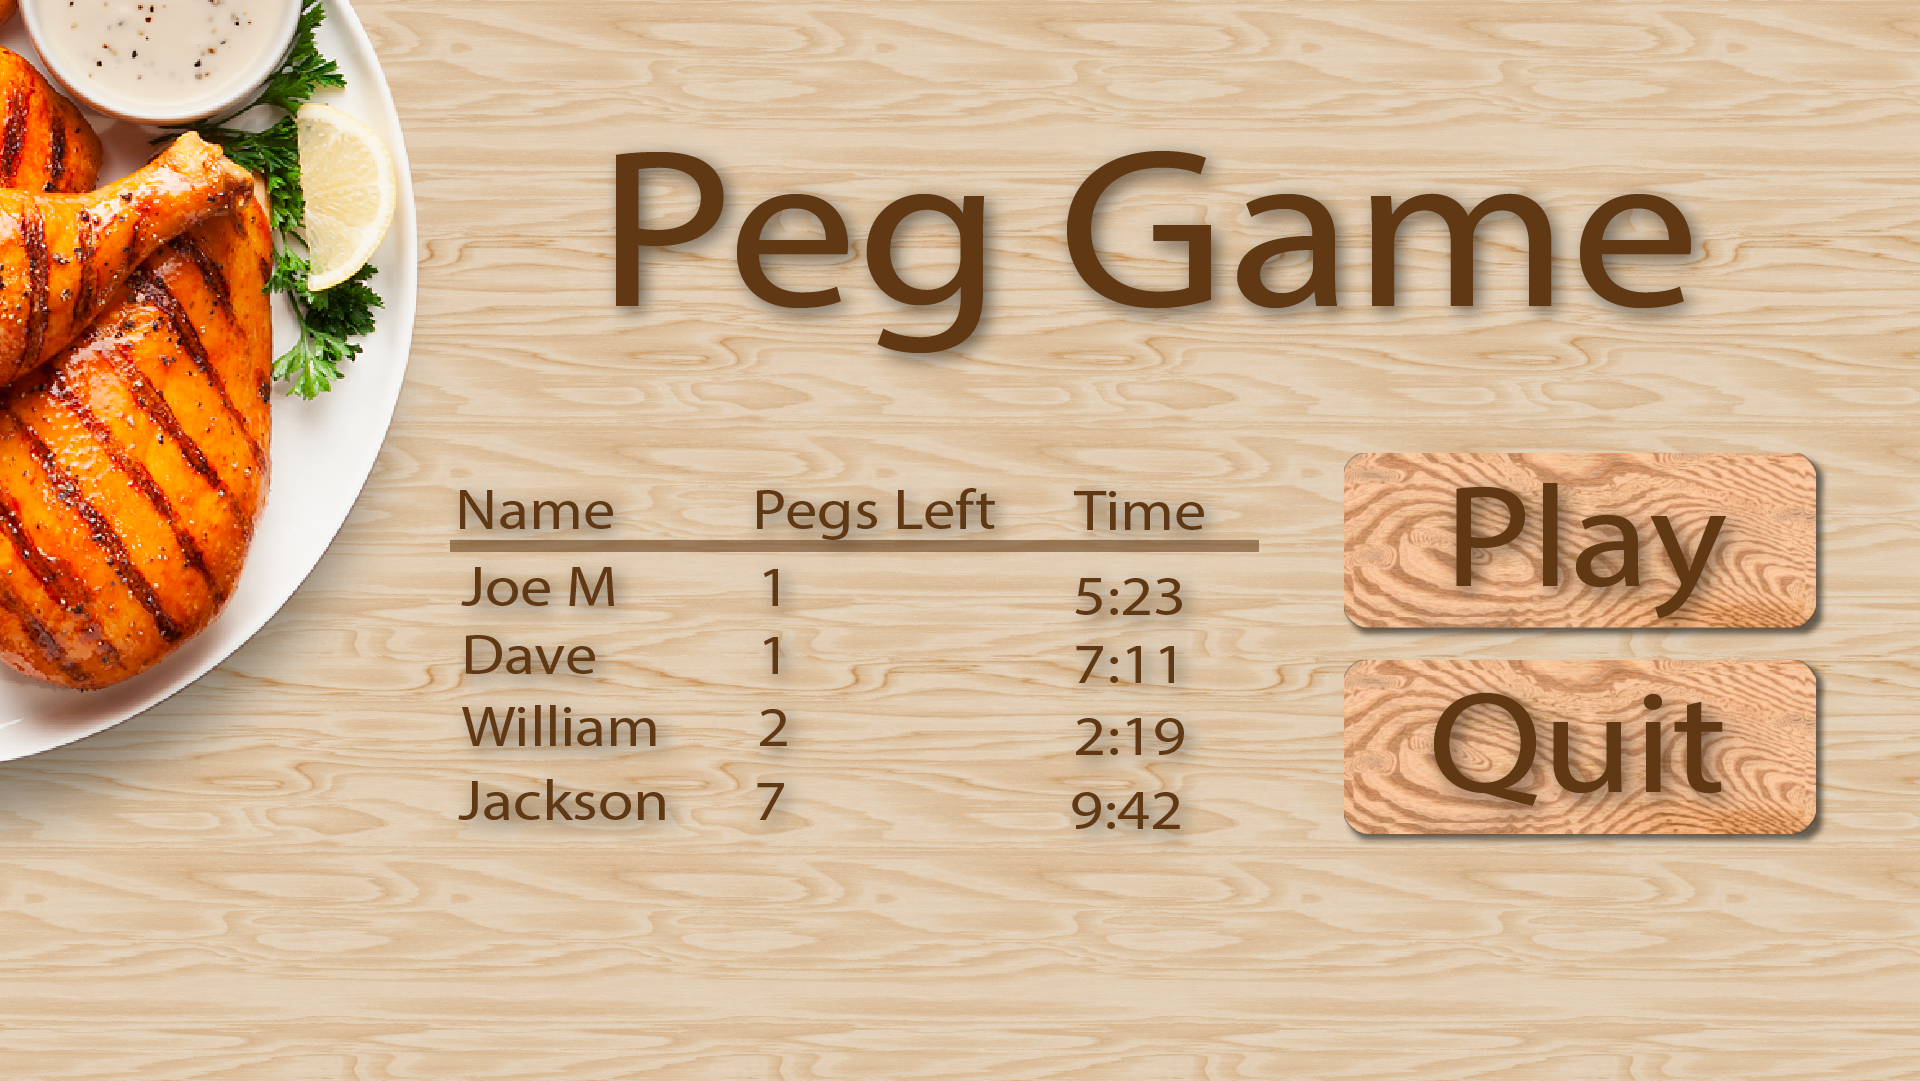
\includegraphics[scale=0.15]{main-menu.png}
        \caption{Mockup of what the main menu will look like with the leaderboard.}
        \label{fig:board-main}
    \end{center}
\end{figure}

This next interface is the gameboard window. Here the player can see and interact with the game board by moving and jumping pegs. Also there are the quit and pause buttons that also the user to quit the game and pause the game respectively. The restart button which generates a new game when clicked on is also available. The user can also click the undo button which undoes previous moves the user made on the game board.

\begin{figure}[H]
    \begin{center}
        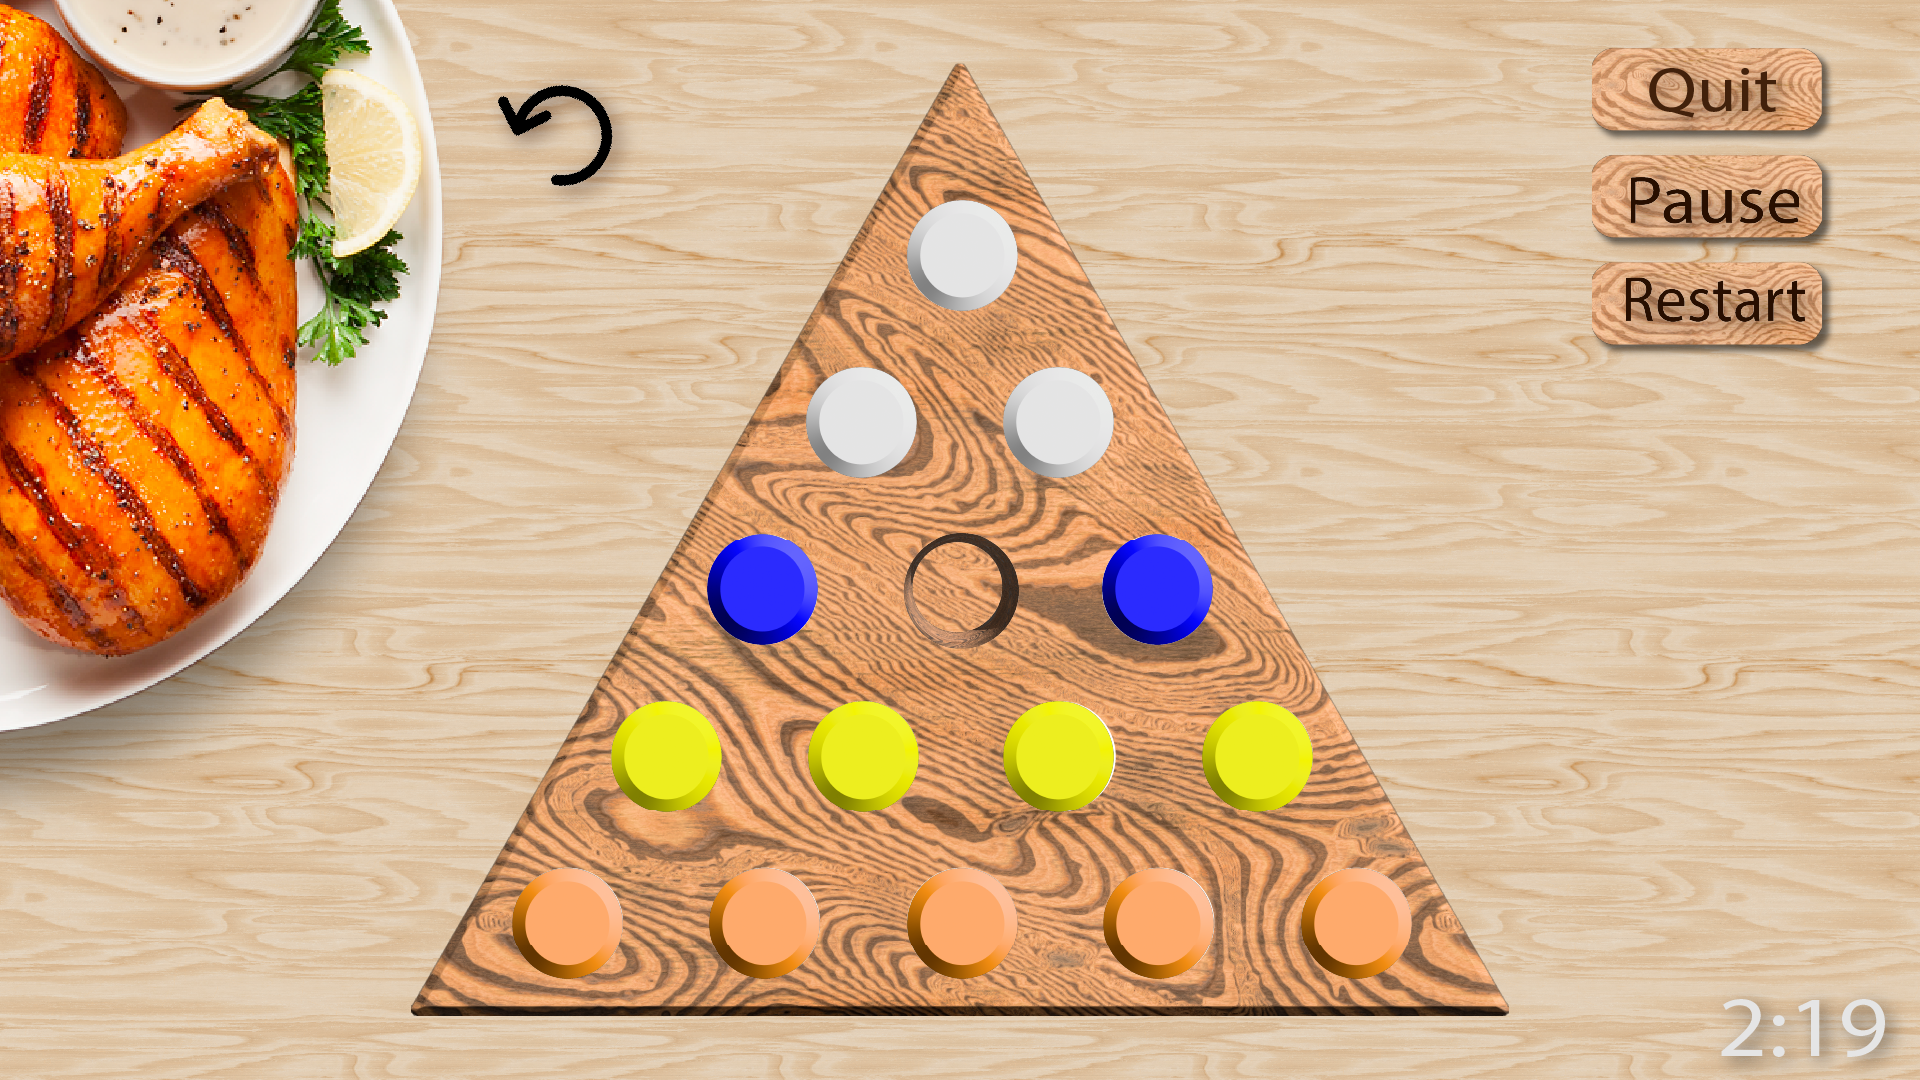
\includegraphics[scale=0.15]{gameplay.png}
        \caption{Mockup of the GUI during gameplay.}
        \label{fig:board-gameplay}
    \end{center}
\end{figure}

Here is the interface for the pause menu, which should suspend the game board window. Available are the resume and quit buttons. The resume should unsuspend the game board window with no changes to the board state or the time lapse since the game's start.

\begin{figure}[H]
    \begin{center}
        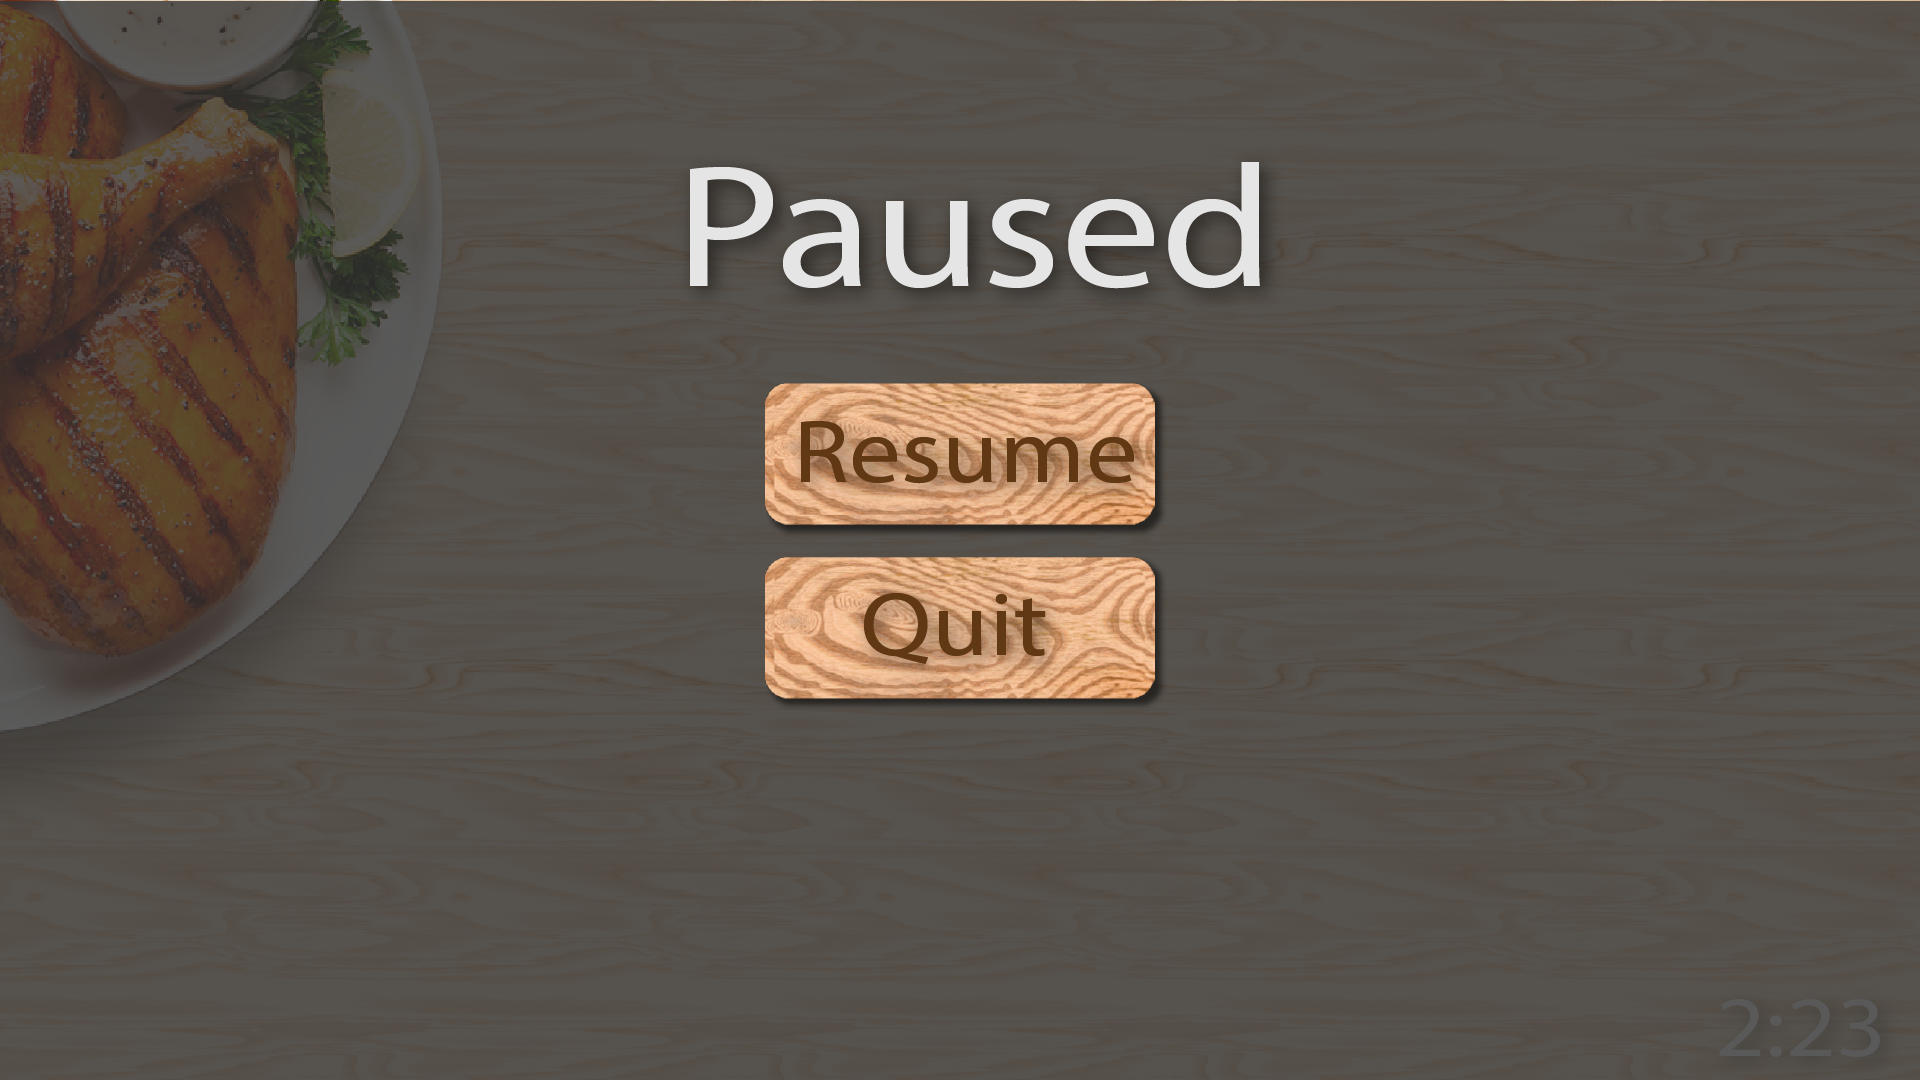
\includegraphics[scale=0.15]{pause-menu.png}
        \caption{Mockup of the pause menu in the GUI.}
        \label{fig:board-pause}
    \end{center}
\end{figure}

\newpage
\section{Project Timeline}
\begin{itemize}
    \item Week 1 (January 8th)- Choose partners for the project.
    \item Week 2 (January 20th)- Came up with idea from the project: creating a peg solitaire game.
    \item Week 3 (January 27th)- Created the GitHub repository and basic requirements for the project.
    \item Week 4 (February 3rd)- Completed the project proposal draft and requirements.
    \item Week 5 (February 10th)- Held project meeting to discuss possible changes and corrections to the draft.
    \item Week 6 (February 17th)- We manage made corrections to the proposal draft and added in some use cases and interface mock-up.
    \item Week 7 (February 24th)- We did plan a meeting to discuss possible design patterns and figure out how make menus on word using grid elements
    \item Week 8 (March 3rd)- Began the implementation stage by creating the hole and peg classes to serve as the project's framework.
    \item Week 9 (March 10th)- Continued to work on project framework. Added in the menu and game board windows and the board class that uses the peg and hole objects.
    \item Week 10 (March 17st)- Made the pegs movable on the board, and created the basic move checker algorithm.
    \item Week 11 (March 31st)- Implemented the game over screen, factory method for button creation, and strategy pattern for the valid move algorithm.
    \item Week 12 (April 7th)- Implemented the undo button, pause button, and the help buttons.
    \item Week 13 (April 12th)- Worked on project presentation and final report.
    \item Week 14 (April 21th)- Implemented the timer and leaderboard stretch goals.
    \item Week 15 (April 28th)- Presented program and its features, and completed the final version of the project report.
\end{itemize}


\section{Project Structure}


\subsection{UML Outline}

\begin{figure}[H]
    \begin{center}
        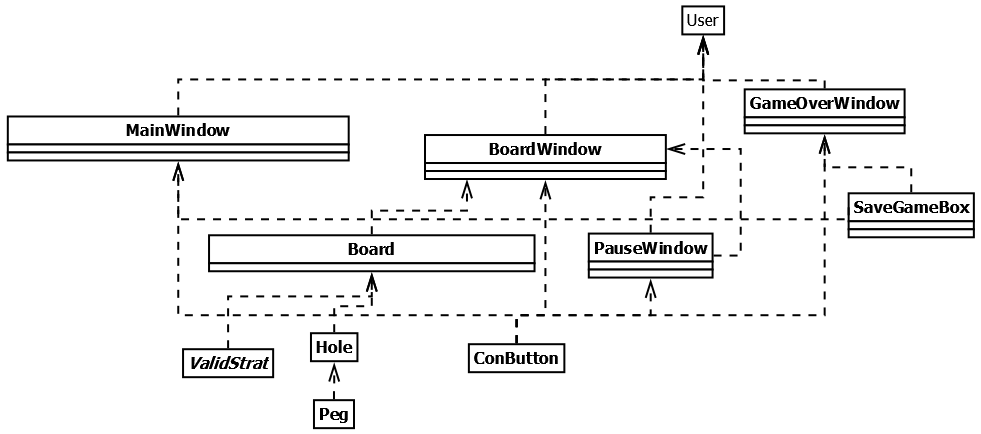
\includegraphics[width=.75\linewidth]{uml.png}
        \caption{UML of the overall project structure.}
        \label{fig:umlstructure}
    \end{center}
\end{figure}


% \begin{figure}[H]
%     \begin{center}
%         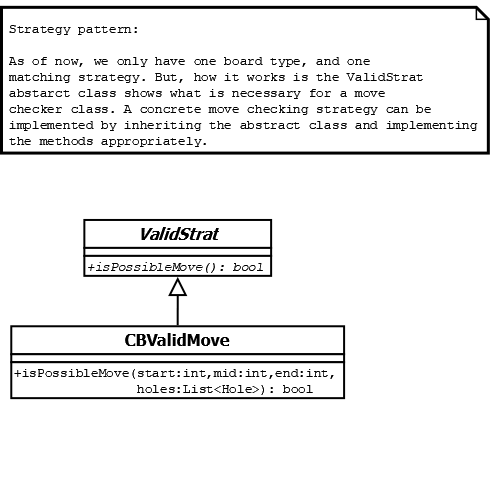
\includegraphics[scale=0.2]{strategy.png}
%         \caption{UML of the strategy pattern.}
%         \label{fig:strategypattern}
%     \end{center}
% \end{figure}

% \begin{figure}[H]
%     \begin{center}
%         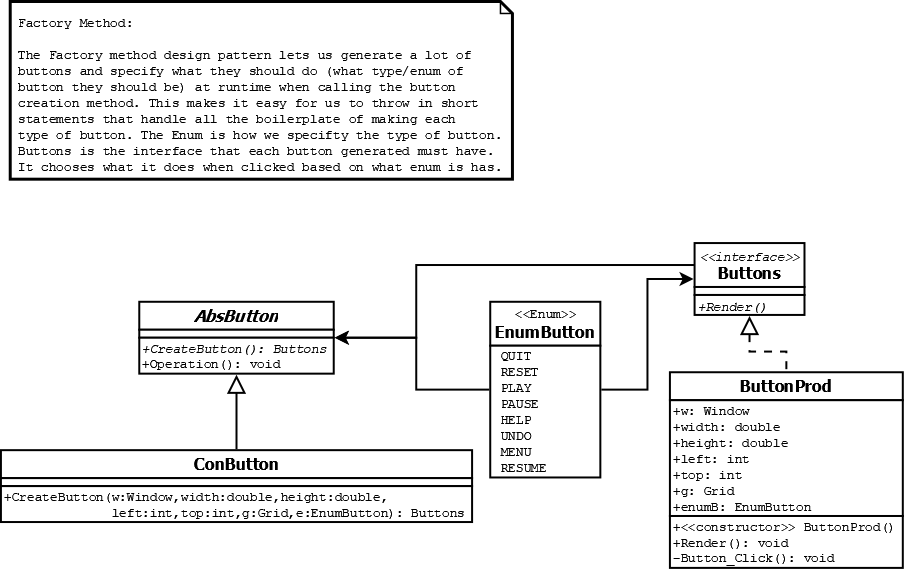
\includegraphics[scale=0.2]{factorymethod.png}
%         \caption{UML of the Factory Method pattern.}
%         \label{fig:factorymethod}
%     \end{center}
% \end{figure}


\begin{figure}[H]
\centering
\begin{subfigure}{.4\textwidth}
  \centering
  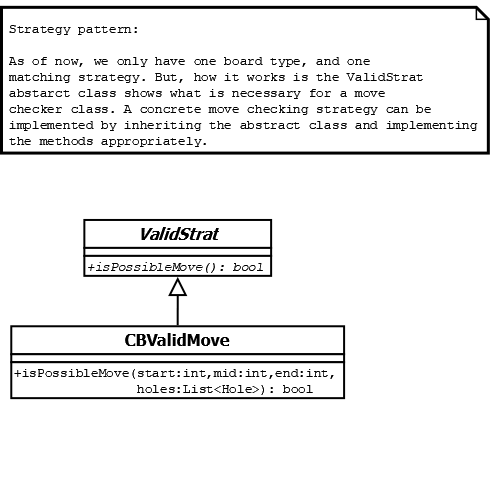
\includegraphics[width=.85\linewidth]{strategy.png}
  \caption{Strategy pattern UML.}
  \label{fig:strategy}
\end{subfigure}%
\begin{subfigure}{.6\textwidth}
  \centering
  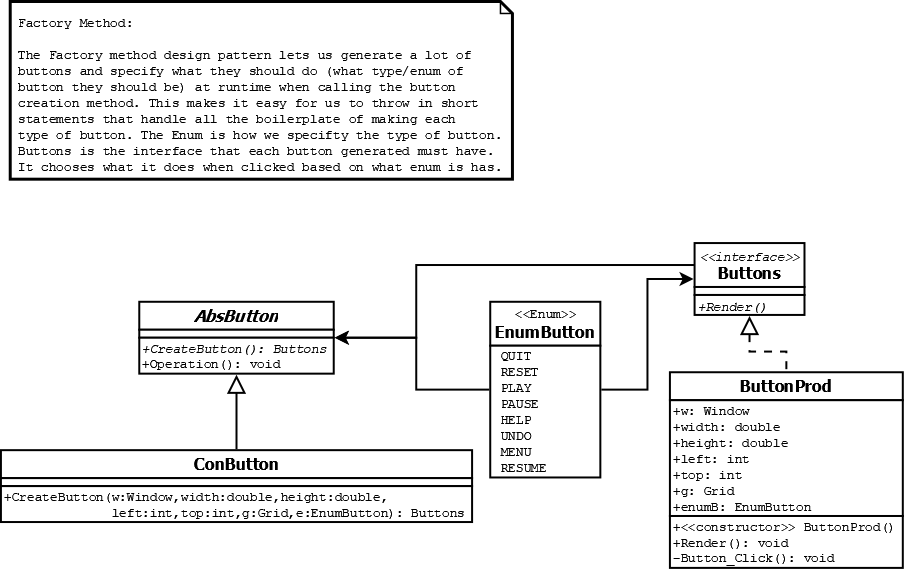
\includegraphics[width=.9\linewidth]{factorymethod.png}
  \caption{Factory Method UML.}
  \label{fig:factory}
\end{subfigure}
\caption{UMLs of the design patterns used in the project.}
\label{fig:patterns}
\end{figure}



\subsection{Design Patterns Used}
\begin{itemize}
    \item \textbf{Factory Method Pattern:} We used a factory method pattern to assist in the creation of button objects. This allowed us to add in multiple button types each with their own individual functionality. Now when we create buttons using the factory method we don't have to rewrite the same boilerplate for each button with the same click event handlers for each type of buttons. 
    \item \textbf{Strategy Pattern:} We used a strategy pattern to allow for the use of different move-checking algorithms at runtime. If we implement additional board shapes and types, they will each require a different algorithm for determining valid moves. Instead of having to revisit the structure of the program when we do add additional boards, we chose to go ahead and implement the strategy pattern. This means when we do possible implement a new board in the future, we just have to create the new valid move class that inherits from the valid move interface.
\end{itemize}

\section{Results}
We started by creating the Peg and Hole classes. Although we planned on the Hole class having the most move functionality (by having this class use the actual valid move checker), we decided to put this logic in the Peg class instead. As a side note, we originally planned on making a factory method for the peg and hole objects, but this was abandoned because we felt that we wanted to implement a lot of the base functionality as quickly as possible to allow us to work more freely after a base had been built.\newline

We also made the board window, which creates the actual game, board, and pieces. This window would later serve as the foundation of our project with everything being slowly built off of it. At this point, we could both work independently and make our own additions on top of the existing code. After the game board was created, we implemented the main menu window. Originally, we planned on creating windows \textit{programmatically} (dynamically with code), but after a week of unsuccessful attempts, we abandoned the programmatic approach for the sake of time. We then developed the logic for moving pegs around using the mouse, jumping/removing pegs, and the valid move checker. \newline

It was extremely difficult because of our lack of experience with WPF and C\#, but we were extremely pleased with the results. Our original idea was a drag-and-drop movement where you could visually move and place the peg where you were moving it. The approach we landed for the sake of simplicity was showing the possible moves with green ellipses when you clicked on a peg; then when you clicked the green ellipse (indicating a possible move), the peg would be moved and remove the jumped peg. It is worth mentioning that we created the strategy pattern to allow us to follow the principle of ETC by allowing for the creation and usage of different valid move-checking algorithms. We also created the factory method to allow for the quick creation of the program's button UI elements. The factory method pattern also helps us maintain the continuity of the look and function of each button. After this, we created the game over screen, adding a main menu, restart, and quit button. \newline

We also added logic that gives the user a little prompt that comments and playfully insults the user based on the number of pegs left on the board. Next, we created the undo button. Originally it was only going to undo one previous move, but after adding a list that stores moves that the user makes, we decided to have it undo any moves the user makes. Recently, we added functionality to the help and pause buttons and created their respective windows. For the pause menu, the difficult part was saving and somehow resuming the game board without changing the state of the board. However, we decided on having the pause button hide the game board window and having a resume button that reveals the game board window. \newline

Our most recent additions are the timer and leaderboard. The timer was developed first and just counts the time since the beginning of the game. We also had to make sure the pause menu stopped the timer. Once we finished the timer and got it to display on the game over window, we had everything we need to implement the leaderboard. We chose to put the leaderboard on the main menu when you open the program. It will sort any stored games by \textbf{1)} the least number of pegs, then by \textbf{2)} the least time taken if two games had equal number of pegs remaining. The user can save their game to the leaderboard by using the save button on the game over screen and entering a name. The top 5 games are shown. We opted to store the games in a text file. We could have used a database, but we chose to just use a local file since \textbf{1)} the data doesn't need to be secure, \textbf{2)} the simplicity of the data (3 attributes), and \textbf{3)} to save system resources and startup time.

\subsection{Future Work}
We were able to implement our requirements and most of our stretch goals. There are certainly some improvements to be made to the look-and-feel of the program, such as the ability to scale the screen. Our final stretch goal to implement would be adding additional boards. As mentioned before, this process should be made easier by already having the strategy pattern pave the way for an easier integration. 

\begin{IEEEbiography}{Michael Shell}
Biography text here.
\end{IEEEbiography}

% if you will not have a photo at all:
\begin{IEEEbiographynophoto}{John Doe}
Biography text here.
\end{IEEEbiographynophoto}

% insert where needed to balance the two columns on the last page with
% biographies
%\newpage

\begin{IEEEbiographynophoto}{Jane Doe}
Biography text here.
\end{IEEEbiographynophoto}





% that's all folks
\end{document}

